\chapter{User Guide}\label{app:user}

This section contains the information necessary to run the optimization.

The software is divided into 3 separate parts:

\begin{itemize}
    \setlength\itemsep{0pt}
    \item Data generation
    \item Optimization algorithms
    \item Results evaluation
\end{itemize}

\section{Prerequisites}

For the \textit{data generation} and \textit{results evaluation} scripts, the user needs
\begin{itemize}
    \setlength\itemsep{0pt}
    \item a Python interpreter in version 3.11.9. Compatibility with different versions is probable but not guaranteed. The libraries needed and their versions are listed in the \textit{requirements.txt} file. 
    \item a running instance of Open Source Routing Machine (OSRM) \cite{luxen-vetter-2011} service. The authors provide a demo server at \texttt{https://router.project-osrm.org}. To host the service, a \textit{Makefile} with \texttt{prepare-server} and \texttt{run-server} targets is prepared in the \textit{osrm} folder in the project files.
\end{itemize}

The \textit{optimization modules} requires a Julia programming language compiler. The program was tested on Julia versions 1.7, 1.8 and 1.9. The packages needed are listed in the \textit{Project.toml} file. The correct environment should be installed by running Julia with the \texttt{-{}-project} argument.

\section{Generating New Instance Data}

The datasets used for running this thesis's experiments are available in the attachments in the \textit{test\_data} folder. If you want to generate new datasets, two scripts are available: \textit{dataGeneratorUniform.py} and \textit{dataGeneratorCommute.py}. Both scripts can be configured using command line arguments, described in detail when running the script with \textit{-{}-help}. Running the script generates a new folder with all the needed files: the \textit{GeoJSON} file with customer requests, \textit{CSV} file with the distance matrix, \textit{CSV} file with the duration matrix and a \textit{parameters.txt} file, where the settings of the generator are stored.

The script assumes that the \textit{OSRM} service runs on your local machine. If your instance runs elsewhere, you can override this with the \texttt{-{}-osrm\_url} option, e.g.

\begin{lstlisting}[language=bash, breaklines=true]
    python dataGeneratorCommute.py --osrm_url https://router.project-osrm.org
\end{lstlisting}

The coordinates used are sampled from public transport platforms in the given area. Note that when generating larger datasets, there must be enough unique platforms to use in that area. If the number of available platforms is lower than what is needed to sample, the generators exit with an error.

The bus type(s) available from the depot are hardcoded in the script. Either change them in the code or afterward in the generated \textit{GeoJSON} file.

\section{Running the optimization algorithms}

All the Julia source files are stored in the \textit{src} folder. Running the algorithms is done using the \textit{EvoDARP.jl} runner script. All hyperparameters and other algorithm configurations are stored in the \textit{config.yaml} file together with their descriptions. The program loads the configuration file from the \textit{src} folder by default, but this can be overridden with the \texttt{--config} option.

The easiest way to run the program is with the following command:
\begin{lstlisting}[language=bash]
    julia EvoDARP.jl
\end{lstlisting}

The command compiles the program, loads the configuration from \textit{config.yaml}, and runs the optimization. If you want to override some configuration variables directly from the command line, you can enter key-value pairs \textit{variable=value} in the command. Some of the examples include:

\begin{lstlisting}[language=bash, breaklines=true]
    julia EvoDARP.jl algorithm=evolution_stops cross_prob=0.5 mut_prob=0.8 num_generations=20000
\end{lstlisting}

\begin{lstlisting}[language=bash, breaklines=true]
    julia EvoDARP.jl input_data_folder=my_data algorithm=aco number_of_runs=10 num_ants=10 num_iterations=10000
\end{lstlisting}

The configuration file is divided into several sections. When running a certain optimization algorithm, all parameters from its section must be present. If some are missing, the program stops and prints an error message describing what is missing.

When the optimization finishes (by reaching maximum iterations or by exceeding the wall time), the runner stores in the output folder the following files:

\begin{itemize}
    \setlength\itemsep{0pt}
    \item \textit{best\_solution.csv} with the overall best solution found.
    \item \textit{config.yaml} with all the hyperparameter settings for the current run. This file can be used to reproduce the experiment.
    \item \textit{run\_$i$.fits}, where $i$ is the run's id for each run, logging the current iteration, time, best fitness, and mean fitness of the population, respectively. Used for creating plots and analyzing the algorithm's convergence. The frequency of the logging can be set in the configuration.
\end{itemize}

The most important configuration values include the following.

\begin{itemize}
    \setlength\itemsep{0pt}
    \item \texttt{algorithm} - which of the algorithms implemented is used for the optimization. Possible values are \textit{evolution\_stops}, \textit{evolution\_cr}, \textit{evolution\_heuristic} and \textit{aco}.
    \item \texttt{input\_data\_folder} - the folder with the instance data. Example datasets are prepared in a \texttt{available\_datasets} dictionary and can be selected by the \textit{chosen\_dataset} parameter. To create valid instance data, use one of the data generators attached. If you want to use your own dataset, it must be stored in a folder containing three files: \textit{data.geojson} file with the customer requests, \textit{distances.csv} file with the distances in meters for all coordinate pairs and \textit{distances.csv} file with the durations in seconds for all the coordinate pairs. The \textit{GeoJSON} file must conform to the JSON schema in Figure~\ref{fig:input_json_schema}.
    \item \texttt{output\_data\_folder} - folder where to store the results.
    \item \texttt{logs\_frequency} - after how many iterations are the log files with best and mean fitnesses updated.
    \item \texttt{number\_of\_runs} - how many times will the algorithm run. All runs have a different random seed. Use the standard Julia \texttt{-{}-threads} command line option to run the runs in parallel.
    \item \texttt{random\_seed} - random seed to use. If not present or if its value is empty, the seed is chosen randomly. If \texttt{number\_of\_runs} is greater than one, each separate run has a seed of \texttt{number\_of\_runs + run\_id}. 
    \item \texttt{wall\_time} - stops the algorithm if it runs for too long. Given in seconds. 
\end{itemize}

\begin{figure}
    \centering
    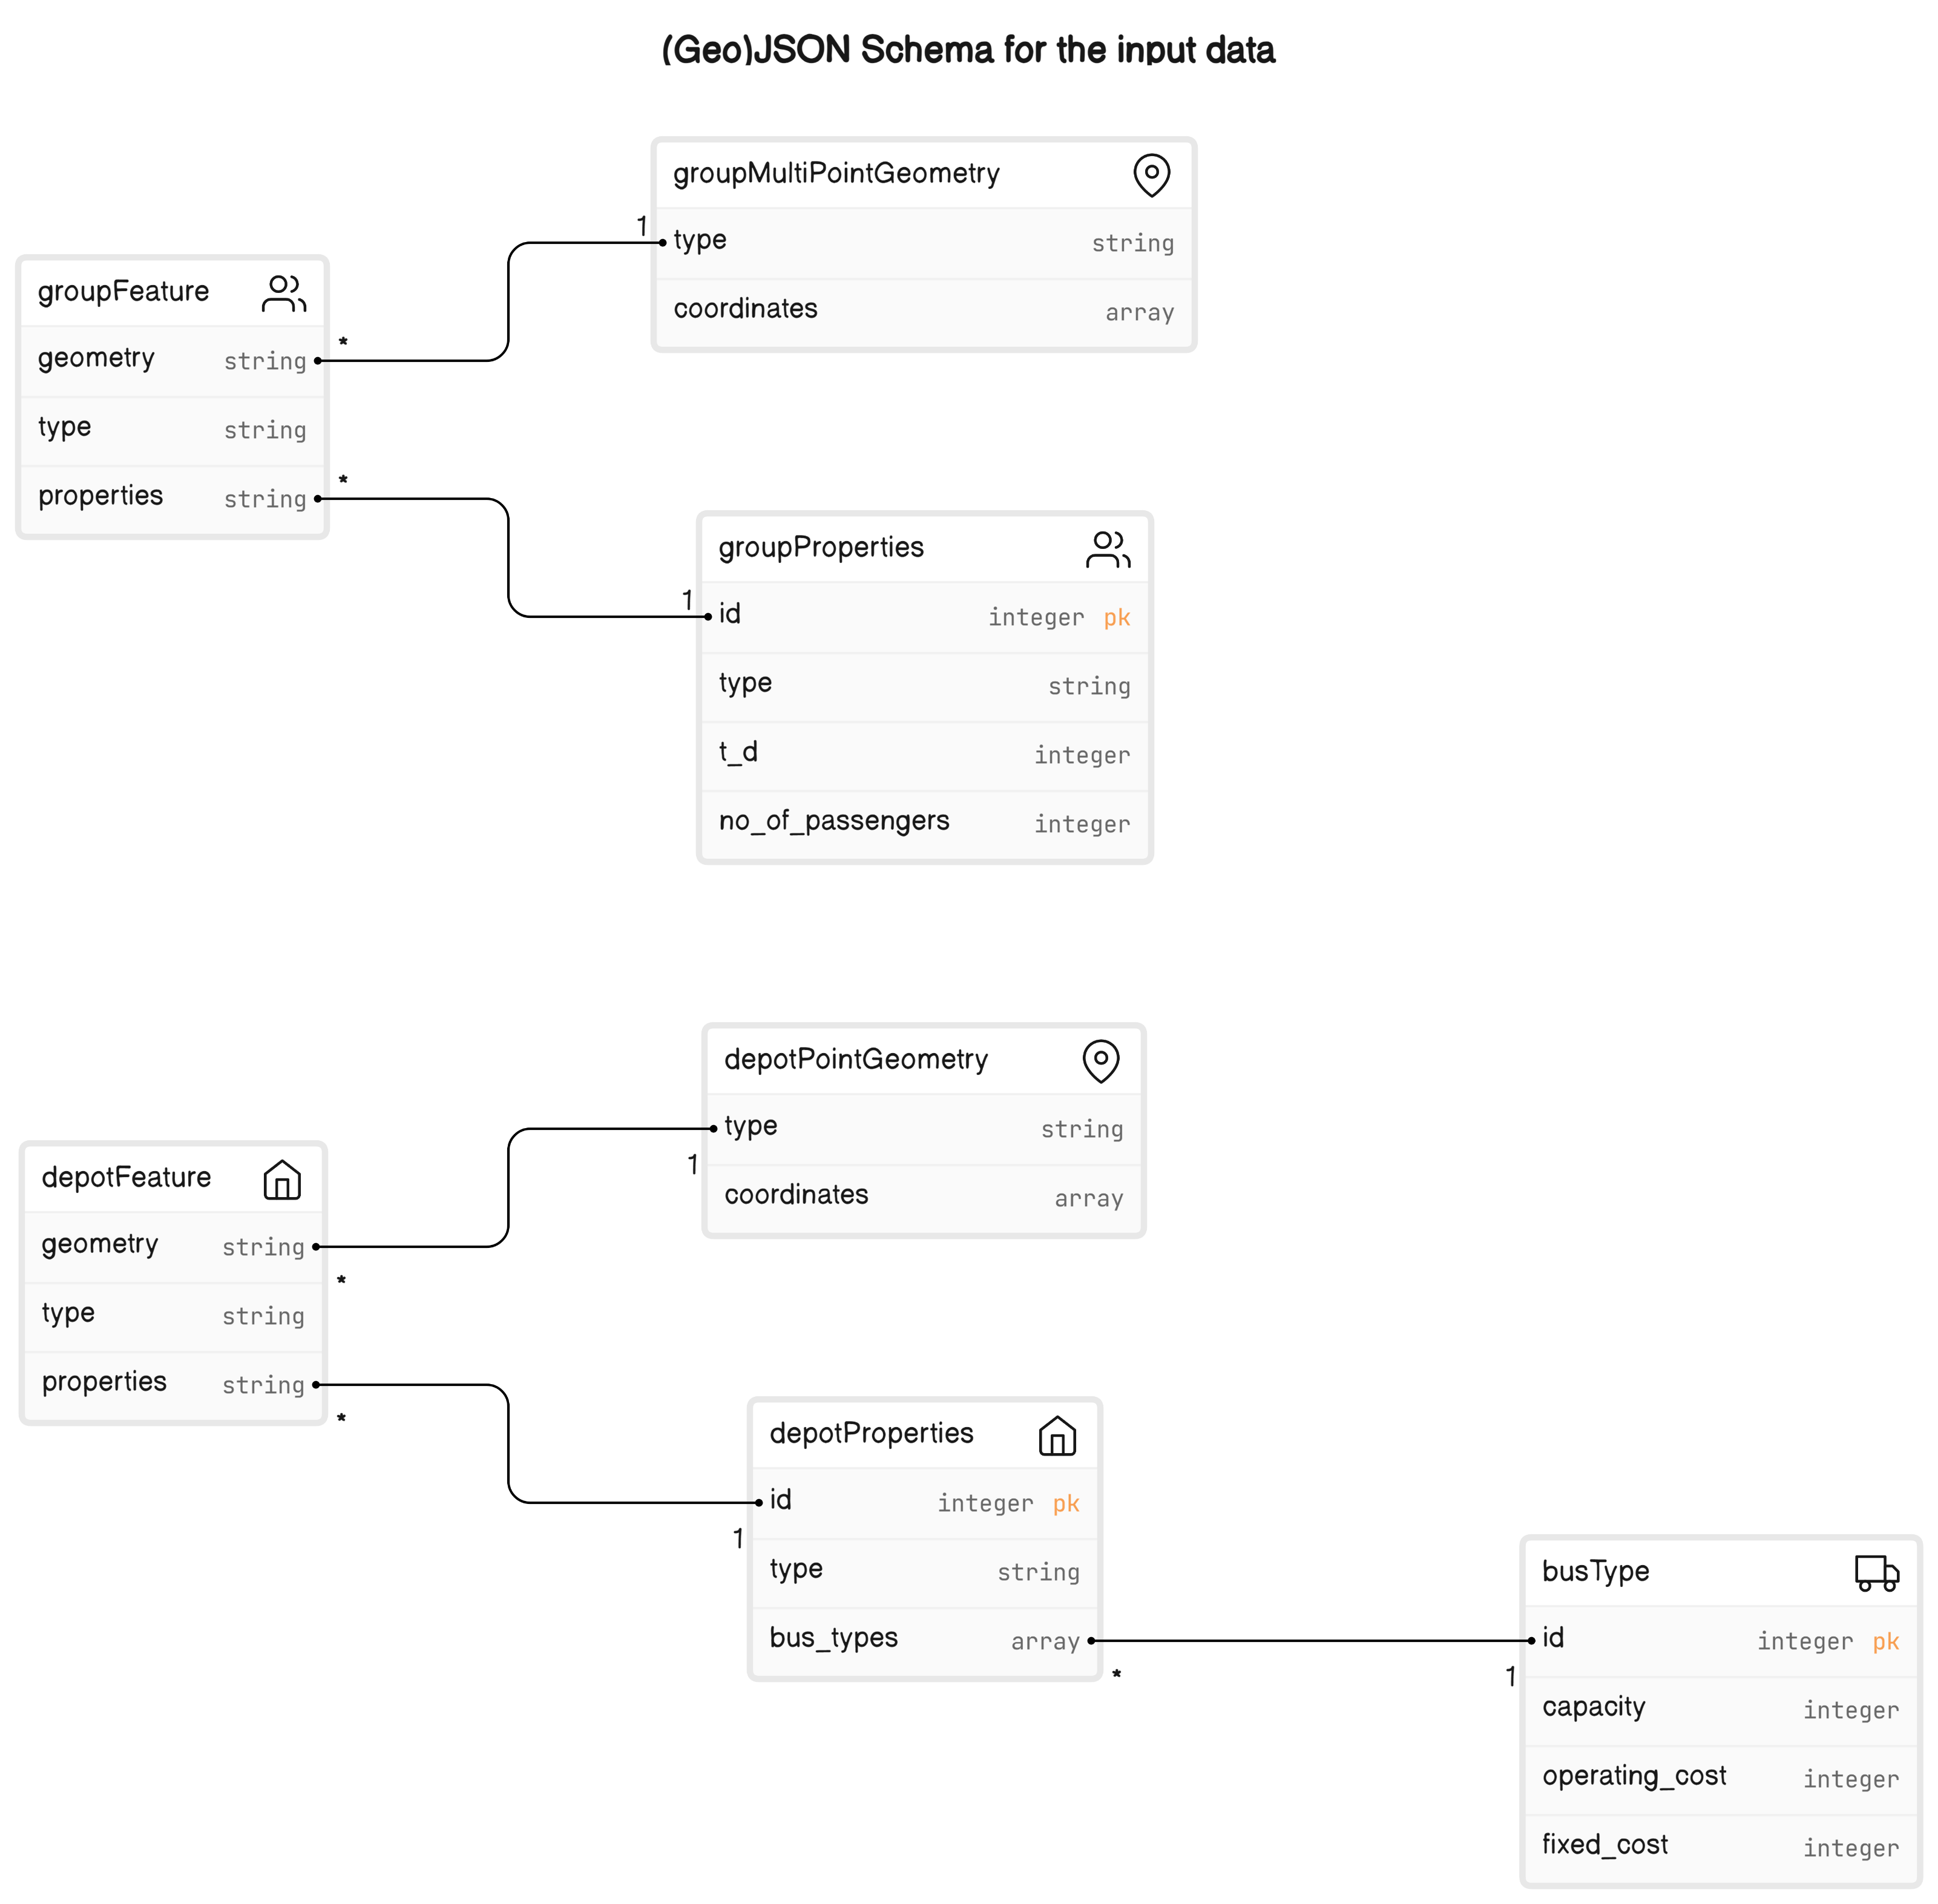
\includegraphics[width=1\linewidth]{img/input_schema_diagram.png}
    \caption{Input GeoJSON schema visualization}
    \label{fig:input_json_schema}
\end{figure}

\section{Parsing the results}

After the optimization finishes, the user can run the \textit{resultsParser.py} script to analyze the results.

The standard way to run the script is with the following command:

\begin{lstlisting}[language=bash]
    python resultsParser.py [-f root_folder] [--visualize]
\end{lstlisting}

The script finds all folders with output from the optimization algorithm within the given folder and creates the following files:

\begin{itemize}
    \setlength\itemsep{0pt}
    \item \textit{report.txt} with basic statistics of the run's best solution, including the total costs, kilometers traveled, individual delays for each group, and the delay's mean and median.
    \item Plots visualizing the progress of the best run and the mean fitness of all the runs. The x-axis in the plots represents the number of generations, and the y-axis represents the fitness.
\end{itemize}

If the \texttt{-v} or \texttt{-{}-visualize} option is used, the script also generates the following files. This option requires the \textit{OSRM} service to be running.

\begin{itemize}
    \setlength\itemsep{0pt}
    \item \textit{routes.geojson} with the routes stored as \textit{LineStrings}. This file can be used with software like \textit{QGIS} to visualize the routes.
    \item \textit{routes.html} with more basic visualization of the routes made with the \textit{Folium} library.
\end{itemize}

To compare multiple experiments and plot them in one figure, use the script with the \texttt{-c} or \texttt{-{}-compare} option:

\begin{lstlisting}[language=bash]
    python resultsParser.py -c [-f results_root_folder] 
\end{lstlisting}

With this option, the script finds all the output folders within the root folder and creates a comparison plot. Again, the plots are generated in 2 variants: with the x-axis representing generations and the x-axis representing time elapsed. The labels in the plot's legend can be set by creating a \textit{legend.txt} file in the experiment's results folder and storing the legend label in it.

There are also \texttt{-{}-xlog} and \texttt{-{}-ylog} options available to set the x-axis or y-axis scale as logarithmic in the plots. For larger experiments, to reduce the size of the plots, the user can use a \texttt{-{}-compress} option. With this option, only points where fitness has changed are plotted.

Similarly to data generation scripts, the default \textit{OSRM} host address can be overridden with the \texttt{-{}-osrm\_url} option.

The project also includes two small scripts to help analyze the results. The \textit{separateCarsDistance.py} script takes 2 command line arguments, a path to a dataset and an output folder, and returns the distances between every group's departure and destination point, and the sum of all the distances. The \textit{greedySpaceTimeHeuristic.py} takes the same 2 command line arguments, as well as additional \texttt{-{}-max\_delay}, \texttt{-{}-travel\_time\_weight} and \texttt{-{}-time\_viol\_weight} arguments. It uses a simple and naive greedy heuristic to find a solution for a given dataset. The heuristic is described in~\ref{experiments-greedy}



